\label{sec: MMO Oscilaltions} %Need this to reference the oscilatory behavious of the system

Before returning to the case of the folded node, a few technical terms are introduced in order to describe the relevant phenomena discussed in this section.
This section is based on work done in the review paper by \citet{MMO} unless indicated otherwise.
The first concept that we need to introduce is mixed mode oscillations (MMOs).

\begin{definition}{\textbf{Mixed Mode Oscillations} \citep{MMO}}\\
	A mixed mode oscillation is an orbit $\gamma$, which traces out small amplitude oscillations (SAOs) as well as large amplitude oscillations (LAOs).
	The SAOs and LAOs are clearly separated in the time series and their recurrence can be periodic.
	The signature of an MMO is expressed as $L_1^{s_1}L_2^{s_2}...$, indicating that $L$ number of LAOs are followed by $s$ SAOs.
\end{definition}
MMOs can be due to different mechanisms in the fast-slow system. They can be present due to a folded node singularity or a singular Hopf bifurcation, amongst others. We can now return to the example of the folded node and state some important results which give rise to MMOs for systems with folded node singularities.

\subsection{The Folded Node}
We have analysed the local behaviour of system (\ref{normalform2}) around the region close to the folded node.
However, this does not provide the full analysis of the system, since the global behaviour of the trajectories that undergo the SAOs in the folded node region is not captured by the local analysis.
Generally, there are no global return mechanisms present in system (\ref{normalform2}) and a trajectory that approaches the folded region from $x = - \infty$ undergoes a number of SAOs, according to where it enters the fold region in $z$ space, before leaving towards infinity. Then there are no global return mechanisms present and the trajectory does not undergo a large amplitude oscillation. However, there are certain criteria that indicate the existence of a global return mechanism and therefore that MMOs can be observed. There are two theorems related to this issue, which are stated below.

\begin{theorem}[\textbf{Generic $1^{k+1}$ MMOs} \citet{MMO}] \label{MMOsigk1}
Consider system (\ref{somegenericthreedim}) with the following assumptions:
\begin{enumerate}
\item Assume that $ 0 < \epsilon \ll 1$ is sufficiently small, $\epsilon^{1/2} \ll \mu$, and $k \in \mathbf{N}$ is such that $2k + 1 < \mu^{-1} < 2k + 3$.
\item The critical manifold $S$ is (locally) a folded surface.
\item The corresponding reduced problem possesses a folded-node singularity.
\item There exists a candidate periodic orbit, which consists of fast fibres of the layer problem, a global return segment, and a segment on $S^a$ within the funnel that starts at distance $\delta$ from $\overline{\gamma_s}$ ( as measured at a distance $O(1)$ away from the fold $F$).
\item An appropriate transversality hypotheses is satisfied.
\end{enumerate}
Then there exists a stable MMO with signature $1^{k+1}$.
\end{theorem}

\begin{theorem}[\textbf{Stable MMOs with signature $1^i$} \citet{MMO}] \label{theoremsigni}
Suppose system (\ref{somegenericthreedim}) satisfies assumptions 1. - 4. of Theorem \ref{MMOsigk1} and, the following additional assumption:
\begin{itemize}
\item For $\delta = 0$, the global return point is on the singular strong canard $\bar{\gamma}_s$ and as $\delta$ passes through zero the return point crosses $\bar{\gamma}_s$ with nonzero speed.
\end{itemize}
Suppose now that $\delta= O(\epsilon ^{(1-\mu)/2})>0$. Then, for sufficiently small $0 < \epsilon \ll 1$ and $k \in \mathbf{N}$ such that $2k+1 < \mu^{-1} < 2k+ 3$, the following holds.
For each $i, 1 \leq i \leq k$, there exist subsectors $\bar{I}_i \subset I_i$ with the corresponding distance intervals $(\delta_i^-, \delta_i^+)$ of widths $O(\epsilon^{(1-\mu)/2})$, which have the property that if $\delta \in (\delta_i^-, \delta_i^+)$, then there exists a stable MMO with signature $1^i$.
\end{theorem}


Theorem \ref{MMOsigk1} is rather technical, stating the existence of the global return under certain circumstances, when the trajectory has entered the rotational sector $I_{k+1}$, meaning, close to the weak primary canard and undergoing $k+1$ SAOs. Since the width of this sector is $O(1)$ and therefore much larger than the width of the other sectors that trajectories can enter into, we would expect more trajectories undergoing $k+1$ SAOs than $i$ SAOs, where $i \in 1,...,k$.
However, Theorem \ref{MMOsigk1} requires $\epsilon^{1/2} \ll \mu$ and since $\epsilon \ll 1$, we must have $\mu \approx 1$ in order to apply the results in this theorem (as $0<\mu<1$). This is not commonly observed in practice and therefore, the logical conclusion is to investigate whether a global return mechanism exists for the other $I_i$, for $i \leq k$. The existence of these MMOs is discussed in Theorem \ref{theoremsigni}. Theorem \ref{theoremsigni} introduces $\delta$ which corresponds to the distance between $\gamma_s$ and the trajectory that has entered the funnel region.\\

As introduced in the beginning of Section \ref{sec:MMO},  the signatures of MMOs are represented in terms of the number of large amplitude oscillations ($L_1L_2...$) and the number of small amplitude oscillations ($s_1s_2\ldots$), and the conventional notation is ($L_1^{s_1}L_2^{s_2}\ldots$).
In the case of the folded node, under the conditions of the theorems, we have a rather straightforward signature. The first theorem states the existence of the signature $1^{k+1}$, where $L_1=1$ and $s^1=k+1$, and equivalently, the second theorem in this chapter discusses MMOs with signature $1^{i}, i<k$.
The dynamics due to a folded node are well understood, however, there exist more complex dynamics for other types of equilibria and singularities.
To illustrate this, one of these cases is briefly introduced in the next section.


\subsection{Singular Hopf Bifurcation}

If the folded singularity is of saddle node type, as introduced in Section \ref{sec: threedimfolds}, there is further classification possible.
There exists the saddle node of type 1, in which the folded singularity coincides with the equilibrium of the desingularised reduced system, which is not the equilibrium of the full system. However, when the parameters of the system coincide in such a way that an equilibrium of the full system and a fold point coincide, then the folded saddle node is said to be of type 2. If a saddle-node of  type 2 occurs for a specific parameter regime, then a singular Hopf bifurcation arises at $O(\epsilon)$ distance from the equilibrium, and is defined as follows:
\begin{definition}{\textbf{Singular Hopf Bifurcation} \citet{strogatz2007nonlinear}}\\
A singular Hopf bifurcation occurs at a certain parameter regime in the system which is $O(\epsilon)$ away from a saddle-node of type 2. There, the eigenvalues of the system cross the imaginary axis, therefore they have a zero real part. Then small oscillations, called limit cycles occur in the system. There are two types of singular Hopf bifurcation. A supercritical Hopf bifurcation occurs when a stable limit cycle arises from an unstable equilibrium point, while a subcritical Hopf bifurcation causes unstable limit cycles to appear around a stable equilibrium.
\end{definition}

A second equilibrium of focus type can appear and interact with the folded saddle node of type 2.
Depending on the parameter regime of the system, this gives rise to various different dynamics.
The normal form which allows for global return mechanisms, due to its S-shaped slow manifold, is the following,
\begin{align*}
\epsilon \dot{x} &= y - x^2 - x^3, \\
\dot{y} &= z - x, \\
\dot{z} &= -\nu -ax -by -cz.
\end{align*}
There exist stable MMOs for some parameter values, where $\nu$ is small and the orbit for a specific choice of such parameters is displayed in Figure \ref{fig: MMo5pic}. Other parameter regimes may give rise to more complex orbits, for example chaotic trajectories that will, with decreasing $\nu$ turn into a small-amplitude chaotic attractor. An example trajectory is displayed in Figure \ref{fig: MMo3pic}, and the time series of this trajectory is displayed in Figure \ref{fig: MMo4pic}. The characterisation of the dynamics of this system for different parameter regimes is still ongoing, and there exist only classifications for certain parameter regimes of $\nu$.
%\begin{figure}[h!]\centering
%	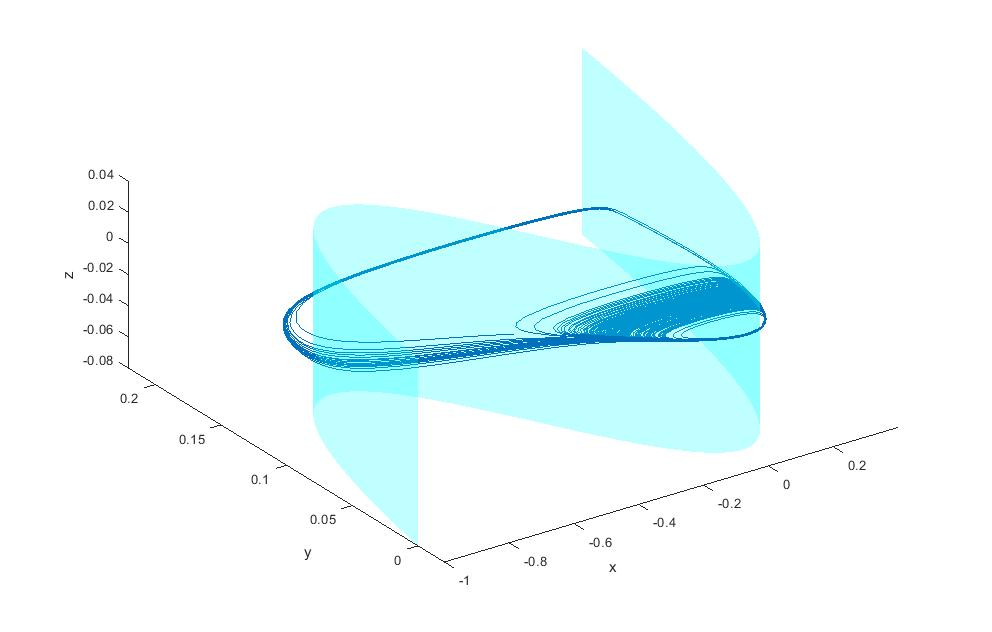
\includegraphics[width= 0.5 \textwidth]{Images/chaoticEvdp}
%	\caption{Chaotic MMO orbit.}
%	\label{fig: MMo3pic}
%\end{figure}
%\begin{figure}[h!]\centering
%	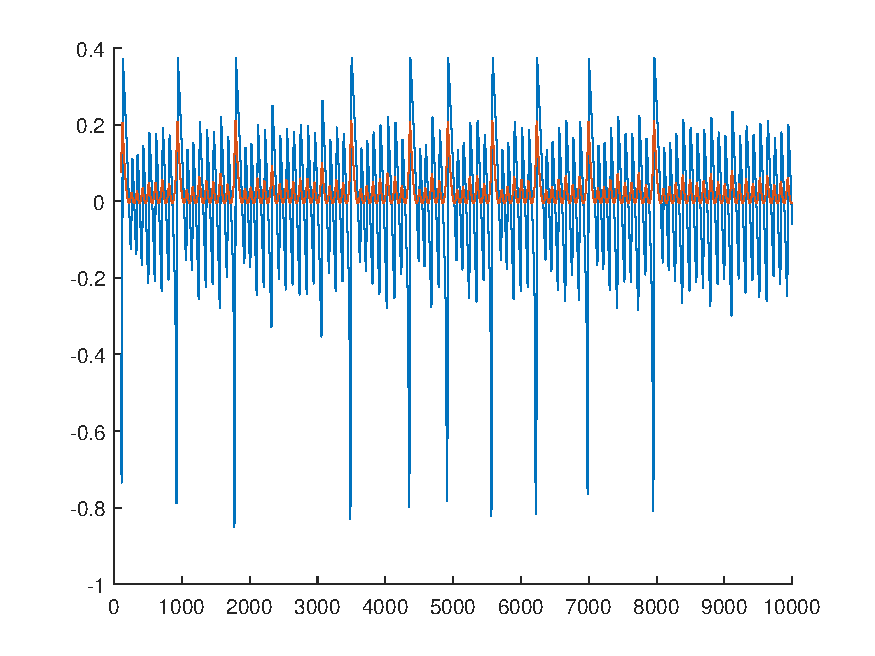
\includegraphics[width= 0.5 \textwidth]{Images/eVDPts}
%	\caption{Time series for the chaotic MMO.}
%	\label{fig: MMo4pic}
%\end{figure}
%\begin{figure}[h!]\centering
%	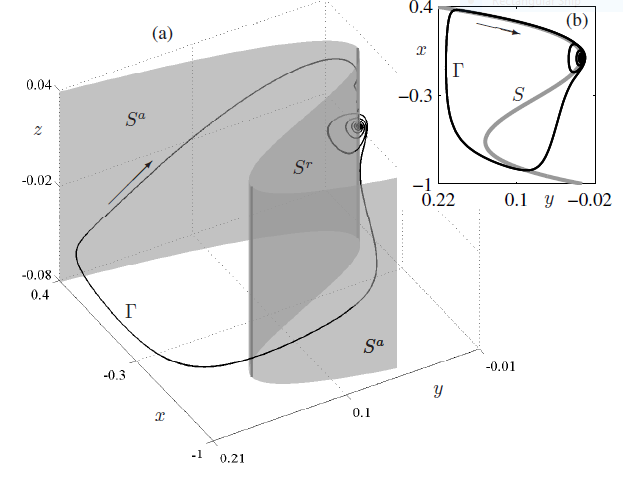
\includegraphics[width= \textwidth]{Images/MMO3}
%	\caption{MMO periodic orbit for $(\nu,a,b,c)= (0.0072168,-0.3872,-0.3251,1.17,0.01)$, \citep{MMO}}
%	\label{fig: MMo5pic}
%\end{figure}


\begin{figure}[h!]
	\centering
	\begin{subfigure}[t]{0.45\textwidth}
		\centering
		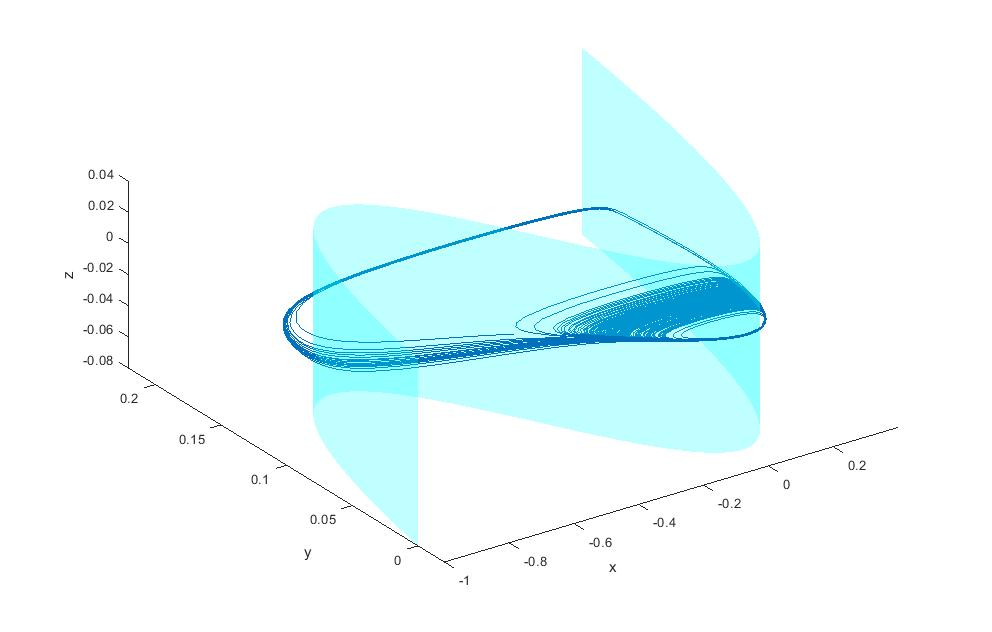
\includegraphics[width=.8\linewidth]{Images/chaoticEvdp}
	\caption{Chaotic MMO orbit.}
	\label{fig: MMo3pic}
	\end{subfigure}
	\hfill
	\begin{subfigure}[t]{0.45\textwidth}
		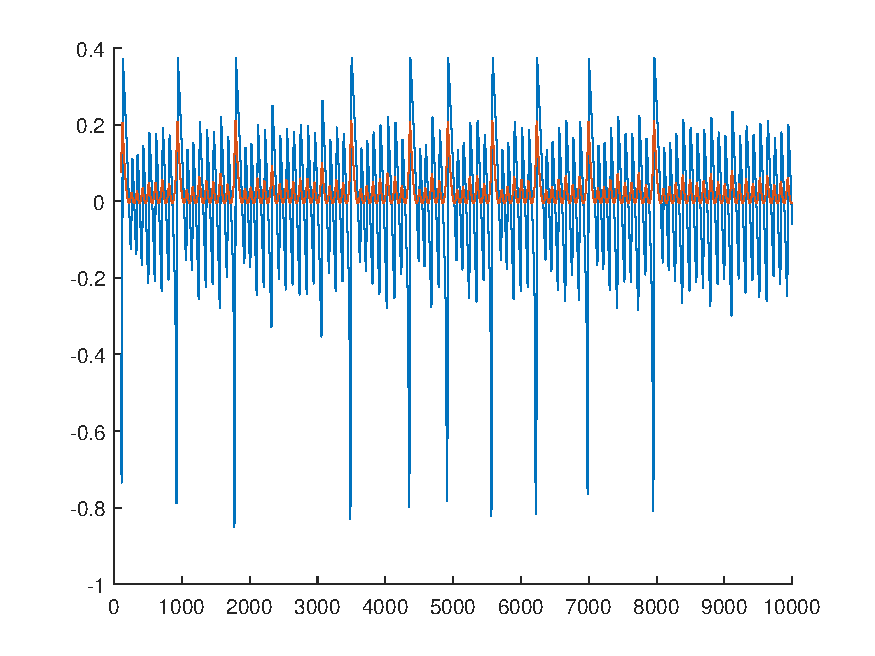
\includegraphics[width=.8\linewidth]{Images/eVDPts}
	\caption{Time series for the chaotic MMO.}
	\label{fig: MMo4pic}
	\end{subfigure}
%	\vspace{1cm}
%\vfill
	\begin{subfigure}[t]{0.45\textwidth}
		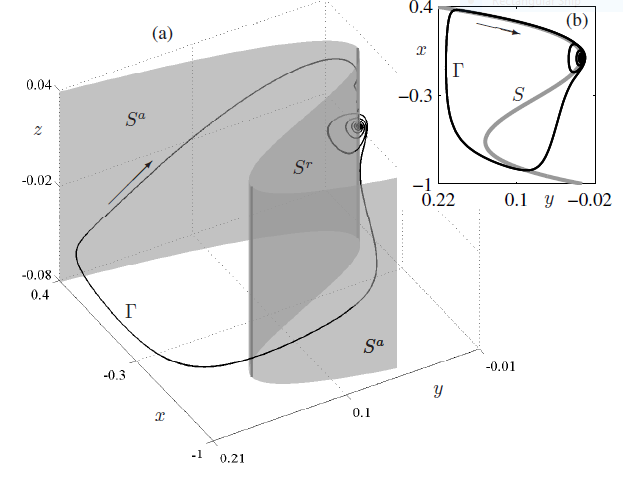
\includegraphics[width=.8\linewidth]{Images/MMO3}
		\caption{MMO periodic orbit for $(\nu,a,b,c)= (0.0072168,-0.3872,-0.3251,1.17,0.01)$, \citep{MMO}.}
		\label{fig: MMo5pic}
	\end{subfigure}
	\caption{Orbits associated with mixed mode oscillations \citep{MMO}.}
\end{figure}\newpage